\documentclass{exam}

\input{preamble.sty}
\begin{document}
\begin{center}
    \Large
\textbf{Lab 7: Multi-Bit Ripple-Carry Adders Workshop}
\end{center}
    \section{4-bit ripple-carry full-adder}
    \subsection{Circuit}
        The flowing circuit is implemented to compute the sum of 2 4-bit numbers (the given one is for 0110 + 1001),
        \begin{center}
                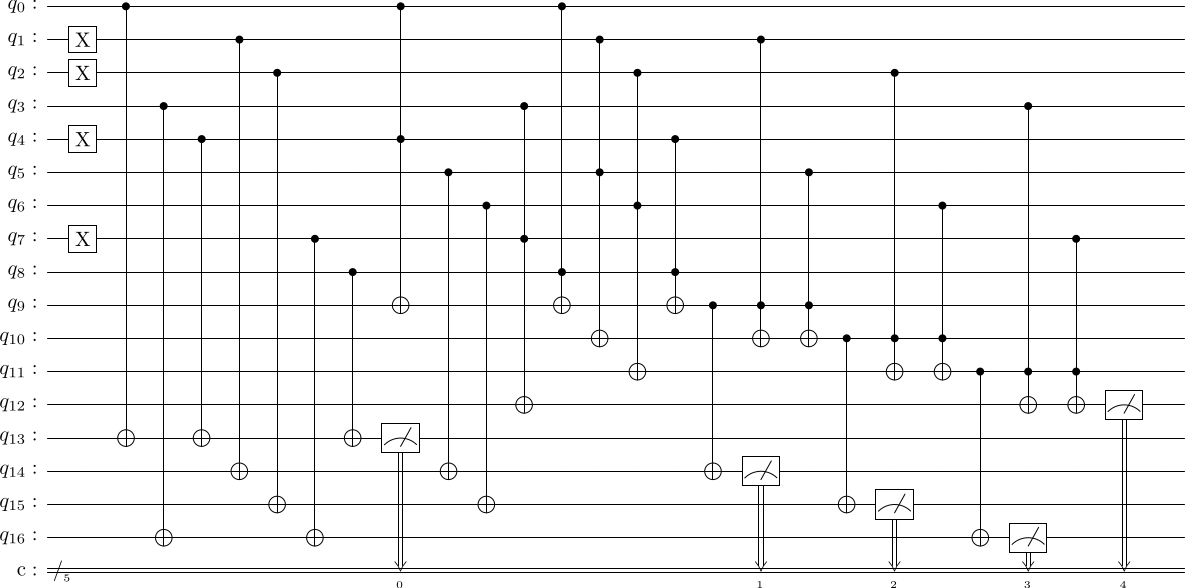
\includegraphics[width = .9 \linewidth]{images/Lab7_4_bit_addr.png}
        \end{center}
        $q_0$ through $q_3$ are used to store $A$.
        $q_4$ through $q_7$ are used to store $B$.
        $q_8$ through $q_{12}$ are used to store the carry from each qubit addition, where $q_8$ is C$_{\text{in}}$.
        $q_{13}$ through $q_{16}$ are used to store the sum from each qubit addition.
        For each carry-bit, a CCNOT gate is used on the A-bit and B-bit, the A-bit and the prevous carry-bit, and the B-bit and the prevous carry-bit.
        For each sum-bit a CNOT gate is used on the A-bit, the B-bit and the carry-bit.
    \subsection{Truth Table}
        The truth table for each possible bit combination is given. The compare row compares adding A and B to the integer representation of the output bit string including the carry.
    \begin{center}
            \begin{longtable}{|c|c|c|c|c|c|}
                \hline
                \textbf{A} & \textbf{B} & \textbf{C$_{\text{in}}$} & \textbf{Sum}& \textbf{C$_{\text{out}}$} & \textbf{Compare}\\ \hline
                0000 & 0000 & 0 & 0000 & 0 & 0 = 0 \\ \hline
                0000 & 0001 & 0 & 0001 & 0 & 1 = 1 \\ \hline
                0000 & 0010 & 0 & 0010 & 0 & 2 = 2 \\ \hline
                0000 & 0011 & 0 & 0011 & 0 & 3 = 3 \\ \hline
                0000 & 0100 & 0 & 0100 & 0 & 4 = 4 \\ \hline
                0000 & 0101 & 0 & 0101 & 0 & 5 = 5 \\ \hline
                0000 & 0110 & 0 & 0110 & 0 & 6 = 6 \\ \hline
                0000 & 0111 & 0 & 0111 & 0 & 7 = 7 \\ \hline
                0000 & 1000 & 0 & 1000 & 0 & 8 = 8 \\ \hline
                0000 & 1001 & 0 & 1001 & 0 & 9 = 9 \\ \hline
                0000 & 1010 & 0 & 1010 & 0 & 10 = 10 \\ \hline
                0000 & 1011 & 0 & 1011 & 0 & 11 = 11 \\ \hline
                0000 & 1100 & 0 & 1100 & 0 & 12 = 12 \\ \hline
                0000 & 1101 & 0 & 1101 & 0 & 13 = 13 \\ \hline
                0000 & 1110 & 0 & 1110 & 0 & 14 = 14 \\ \hline
                0000 & 1111 & 0 & 1111 & 0 & 15 = 15 \\ \hline
                0001 & 0000 & 0 & 0001 & 0 & 1 = 1 \\ \hline
                0001 & 0001 & 0 & 0010 & 0 & 2 = 2 \\ \hline
                0001 & 0010 & 0 & 0011 & 0 & 3 = 3 \\ \hline
                0001 & 0011 & 0 & 0100 & 0 & 4 = 4 \\ \hline
                0001 & 0100 & 0 & 0101 & 0 & 5 = 5 \\ \hline
                0001 & 0101 & 0 & 0110 & 0 & 6 = 6 \\ \hline
                0001 & 0110 & 0 & 0111 & 0 & 7 = 7 \\ \hline
                0001 & 0111 & 0 & 1000 & 0 & 8 = 8 \\ \hline
                0001 & 1000 & 0 & 1001 & 0 & 9 = 9 \\ \hline
                0001 & 1001 & 0 & 1010 & 0 & 10 = 10 \\ \hline
                0001 & 1010 & 0 & 1011 & 0 & 11 = 11 \\ \hline
                0001 & 1011 & 0 & 1100 & 0 & 12 = 12 \\ \hline
                0001 & 1100 & 0 & 1101 & 0 & 13 = 13 \\ \hline
                0001 & 1101 & 0 & 1110 & 0 & 14 = 14 \\ \hline
                0001 & 1110 & 0 & 1111 & 0 & 15 = 15 \\ \hline
                0001 & 1111 & 0 & 0000 & 1 & 16 = 16 \\ \hline
                0010 & 0000 & 0 & 0010 & 0 & 2 = 2 \\ \hline
                0010 & 0001 & 0 & 0011 & 0 & 3 = 3 \\ \hline
                0010 & 0010 & 0 & 0100 & 0 & 4 = 4 \\ \hline
                0010 & 0011 & 0 & 0101 & 0 & 5 = 5 \\ \hline
                0010 & 0100 & 0 & 0110 & 0 & 6 = 6 \\ \hline
                0010 & 0101 & 0 & 0111 & 0 & 7 = 7 \\ \hline
                0010 & 0110 & 0 & 1000 & 0 & 8 = 8 \\ \hline
                0010 & 0111 & 0 & 1001 & 0 & 9 = 9 \\ \hline
                0010 & 1000 & 0 & 1010 & 0 & 10 = 10 \\ \hline
                0010 & 1001 & 0 & 1011 & 0 & 11 = 11 \\ \hline
                0010 & 1010 & 0 & 1100 & 0 & 12 = 12 \\ \hline
                0010 & 1011 & 0 & 1101 & 0 & 13 = 13 \\ \hline
                0010 & 1100 & 0 & 1110 & 0 & 14 = 14 \\ \hline
                0010 & 1101 & 0 & 1111 & 0 & 15 = 15 \\ \hline
                0010 & 1110 & 0 & 0000 & 1 & 16 = 16 \\ \hline
                0010 & 1111 & 0 & 0001 & 1 & 17 = 17 \\ \hline
                0011 & 0000 & 0 & 0011 & 0 & 3 = 3 \\ \hline
                0011 & 0001 & 0 & 0100 & 0 & 4 = 4 \\ \hline
                0011 & 0010 & 0 & 0101 & 0 & 5 = 5 \\ \hline
                0011 & 0011 & 0 & 0110 & 0 & 6 = 6 \\ \hline
                0011 & 0100 & 0 & 0111 & 0 & 7 = 7 \\ \hline
                0011 & 0101 & 0 & 1000 & 0 & 8 = 8 \\ \hline
                0011 & 0110 & 0 & 1001 & 0 & 9 = 9 \\ \hline
                0011 & 0111 & 0 & 1010 & 0 & 10 = 10 \\ \hline
                0011 & 1000 & 0 & 1011 & 0 & 11 = 11 \\ \hline
                0011 & 1001 & 0 & 1100 & 0 & 12 = 12 \\ \hline
                0011 & 1010 & 0 & 1101 & 0 & 13 = 13 \\ \hline
                0011 & 1011 & 0 & 1110 & 0 & 14 = 14 \\ \hline
                0011 & 1100 & 0 & 1111 & 0 & 15 = 15 \\ \hline
                0011 & 1101 & 0 & 0000 & 1 & 16 = 16 \\ \hline
                0011 & 1110 & 0 & 0001 & 1 & 17 = 17 \\ \hline
                0011 & 1111 & 0 & 0010 & 1 & 18 = 18 \\ \hline
                0100 & 0000 & 0 & 0100 & 0 & 4 = 4 \\ \hline
                0100 & 0001 & 0 & 0101 & 0 & 5 = 5 \\ \hline
                0100 & 0010 & 0 & 0110 & 0 & 6 = 6 \\ \hline
                0100 & 0011 & 0 & 0111 & 0 & 7 = 7 \\ \hline
                0100 & 0100 & 0 & 1000 & 0 & 8 = 8 \\ \hline
                0100 & 0101 & 0 & 1001 & 0 & 9 = 9 \\ \hline
                0100 & 0110 & 0 & 1010 & 0 & 10 = 10 \\ \hline
                0100 & 0111 & 0 & 1011 & 0 & 11 = 11 \\ \hline
                0100 & 1000 & 0 & 1100 & 0 & 12 = 12 \\ \hline
                0100 & 1001 & 0 & 1101 & 0 & 13 = 13 \\ \hline
                0100 & 1010 & 0 & 1110 & 0 & 14 = 14 \\ \hline
                0100 & 1011 & 0 & 1111 & 0 & 15 = 15 \\ \hline
                0100 & 1100 & 0 & 0000 & 1 & 16 = 16 \\ \hline
                0100 & 1101 & 0 & 0001 & 1 & 17 = 17 \\ \hline
                0100 & 1110 & 0 & 0010 & 1 & 18 = 18 \\ \hline
                0100 & 1111 & 0 & 0011 & 1 & 19 = 19 \\ \hline
                0101 & 0000 & 0 & 0101 & 0 & 5 = 5 \\ \hline
                0101 & 0001 & 0 & 0110 & 0 & 6 = 6 \\ \hline
                0101 & 0010 & 0 & 0111 & 0 & 7 = 7 \\ \hline
                0101 & 0011 & 0 & 1000 & 0 & 8 = 8 \\ \hline
                0101 & 0100 & 0 & 1001 & 0 & 9 = 9 \\ \hline
                0101 & 0101 & 0 & 1010 & 0 & 10 = 10 \\ \hline
                0101 & 0110 & 0 & 1011 & 0 & 11 = 11 \\ \hline
                0101 & 0111 & 0 & 1100 & 0 & 12 = 12 \\ \hline
                0101 & 1000 & 0 & 1101 & 0 & 13 = 13 \\ \hline
                0101 & 1001 & 0 & 1110 & 0 & 14 = 14 \\ \hline
                0101 & 1010 & 0 & 1111 & 0 & 15 = 15 \\ \hline
                0101 & 1011 & 0 & 0000 & 1 & 16 = 16 \\ \hline
                0101 & 1100 & 0 & 0001 & 1 & 17 = 17 \\ \hline
                0101 & 1101 & 0 & 0010 & 1 & 18 = 18 \\ \hline
                0101 & 1110 & 0 & 0011 & 1 & 19 = 19 \\ \hline
                0101 & 1111 & 0 & 0100 & 1 & 20 = 20 \\ \hline
                0110 & 0000 & 0 & 0110 & 0 & 6 = 6 \\ \hline
                0110 & 0001 & 0 & 0111 & 0 & 7 = 7 \\ \hline
                0110 & 0010 & 0 & 1000 & 0 & 8 = 8 \\ \hline
                0110 & 0011 & 0 & 1001 & 0 & 9 = 9 \\ \hline
                0110 & 0100 & 0 & 1010 & 0 & 10 = 10 \\ \hline
                0110 & 0101 & 0 & 1011 & 0 & 11 = 11 \\ \hline
                0110 & 0110 & 0 & 1100 & 0 & 12 = 12 \\ \hline
                0110 & 0111 & 0 & 1101 & 0 & 13 = 13 \\ \hline
                0110 & 1000 & 0 & 1110 & 0 & 14 = 14 \\ \hline
                0110 & 1001 & 0 & 1111 & 0 & 15 = 15 \\ \hline
                0110 & 1010 & 0 & 0000 & 1 & 16 = 16 \\ \hline
                0110 & 1011 & 0 & 0001 & 1 & 17 = 17 \\ \hline
                0110 & 1100 & 0 & 0010 & 1 & 18 = 18 \\ \hline
                0110 & 1101 & 0 & 0011 & 1 & 19 = 19 \\ \hline
                0110 & 1110 & 0 & 0100 & 1 & 20 = 20 \\ \hline
                0110 & 1111 & 0 & 0101 & 1 & 21 = 21 \\ \hline
                0111 & 0000 & 0 & 0111 & 0 & 7 = 7 \\ \hline
                0111 & 0001 & 0 & 1000 & 0 & 8 = 8 \\ \hline
                0111 & 0010 & 0 & 1001 & 0 & 9 = 9 \\ \hline
                0111 & 0011 & 0 & 1010 & 0 & 10 = 10 \\ \hline
                0111 & 0100 & 0 & 1011 & 0 & 11 = 11 \\ \hline
                0111 & 0101 & 0 & 1100 & 0 & 12 = 12 \\ \hline
                0111 & 0110 & 0 & 1101 & 0 & 13 = 13 \\ \hline
                0111 & 0111 & 0 & 1110 & 0 & 14 = 14 \\ \hline
                0111 & 1000 & 0 & 1111 & 0 & 15 = 15 \\ \hline
                0111 & 1001 & 0 & 0000 & 1 & 16 = 16 \\ \hline
                0111 & 1010 & 0 & 0001 & 1 & 17 = 17 \\ \hline
                0111 & 1011 & 0 & 0010 & 1 & 18 = 18 \\ \hline
                0111 & 1100 & 0 & 0011 & 1 & 19 = 19 \\ \hline
                0111 & 1101 & 0 & 0100 & 1 & 20 = 20 \\ \hline
                0111 & 1110 & 0 & 0101 & 1 & 21 = 21 \\ \hline
                0111 & 1111 & 0 & 0110 & 1 & 22 = 22 \\ \hline
                1000 & 0000 & 0 & 1000 & 0 & 8 = 8 \\ \hline
                1000 & 0001 & 0 & 1001 & 0 & 9 = 9 \\ \hline
                1000 & 0010 & 0 & 1010 & 0 & 10 = 10 \\ \hline
                1000 & 0011 & 0 & 1011 & 0 & 11 = 11 \\ \hline
                1000 & 0100 & 0 & 1100 & 0 & 12 = 12 \\ \hline
                1000 & 0101 & 0 & 1101 & 0 & 13 = 13 \\ \hline
                1000 & 0110 & 0 & 1110 & 0 & 14 = 14 \\ \hline
                1000 & 0111 & 0 & 1111 & 0 & 15 = 15 \\ \hline
                1000 & 1000 & 0 & 0000 & 1 & 16 = 16 \\ \hline
                1000 & 1001 & 0 & 0001 & 1 & 17 = 17 \\ \hline
                1000 & 1010 & 0 & 0010 & 1 & 18 = 18 \\ \hline
                1000 & 1011 & 0 & 0011 & 1 & 19 = 19 \\ \hline
                1000 & 1100 & 0 & 0100 & 1 & 20 = 20 \\ \hline
                1000 & 1101 & 0 & 0101 & 1 & 21 = 21 \\ \hline
                1000 & 1110 & 0 & 0110 & 1 & 22 = 22 \\ \hline
                1000 & 1111 & 0 & 0111 & 1 & 23 = 23 \\ \hline
                1001 & 0000 & 0 & 1001 & 0 & 9 = 9 \\ \hline
                1001 & 0001 & 0 & 1010 & 0 & 10 = 10 \\ \hline
                1001 & 0010 & 0 & 1011 & 0 & 11 = 11 \\ \hline
                1001 & 0011 & 0 & 1100 & 0 & 12 = 12 \\ \hline
                1001 & 0100 & 0 & 1101 & 0 & 13 = 13 \\ \hline
                1001 & 0101 & 0 & 1110 & 0 & 14 = 14 \\ \hline
                1001 & 0110 & 0 & 1111 & 0 & 15 = 15 \\ \hline
                1001 & 0111 & 0 & 0000 & 1 & 16 = 16 \\ \hline
                1001 & 1000 & 0 & 0001 & 1 & 17 = 17 \\ \hline
                1001 & 1001 & 0 & 0010 & 1 & 18 = 18 \\ \hline
                1001 & 1010 & 0 & 0011 & 1 & 19 = 19 \\ \hline
                1001 & 1011 & 0 & 0100 & 1 & 20 = 20 \\ \hline
                1001 & 1100 & 0 & 0101 & 1 & 21 = 21 \\ \hline
                1001 & 1101 & 0 & 0110 & 1 & 22 = 22 \\ \hline
                1001 & 1110 & 0 & 0111 & 1 & 23 = 23 \\ \hline
                1001 & 1111 & 0 & 1000 & 1 & 24 = 24 \\ \hline
                1010 & 0000 & 0 & 1010 & 0 & 10 = 10 \\ \hline
                1010 & 0001 & 0 & 1011 & 0 & 11 = 11 \\ \hline
                1010 & 0010 & 0 & 1100 & 0 & 12 = 12 \\ \hline
                1010 & 0011 & 0 & 1101 & 0 & 13 = 13 \\ \hline
                1010 & 0100 & 0 & 1110 & 0 & 14 = 14 \\ \hline
                1010 & 0101 & 0 & 1111 & 0 & 15 = 15 \\ \hline
                1010 & 0110 & 0 & 0000 & 1 & 16 = 16 \\ \hline
                1010 & 0111 & 0 & 0001 & 1 & 17 = 17 \\ \hline
                1010 & 1000 & 0 & 0010 & 1 & 18 = 18 \\ \hline
                1010 & 1001 & 0 & 0011 & 1 & 19 = 19 \\ \hline
                1010 & 1010 & 0 & 0100 & 1 & 20 = 20 \\ \hline
                1010 & 1011 & 0 & 0101 & 1 & 21 = 21 \\ \hline
                1010 & 1100 & 0 & 0110 & 1 & 22 = 22 \\ \hline
                1010 & 1101 & 0 & 0111 & 1 & 23 = 23 \\ \hline
                1010 & 1110 & 0 & 1000 & 1 & 24 = 24 \\ \hline
                1010 & 1111 & 0 & 1001 & 1 & 25 = 25 \\ \hline
                1011 & 0000 & 0 & 1011 & 0 & 11 = 11 \\ \hline
                1011 & 0001 & 0 & 1100 & 0 & 12 = 12 \\ \hline
                1011 & 0010 & 0 & 1101 & 0 & 13 = 13 \\ \hline
                1011 & 0011 & 0 & 1110 & 0 & 14 = 14 \\ \hline
                1011 & 0100 & 0 & 1111 & 0 & 15 = 15 \\ \hline
                1011 & 0101 & 0 & 0000 & 1 & 16 = 16 \\ \hline
                1011 & 0110 & 0 & 0001 & 1 & 17 = 17 \\ \hline
                1011 & 0111 & 0 & 0010 & 1 & 18 = 18 \\ \hline
                1011 & 1000 & 0 & 0011 & 1 & 19 = 19 \\ \hline
                1011 & 1001 & 0 & 0100 & 1 & 20 = 20 \\ \hline
                1011 & 1010 & 0 & 0101 & 1 & 21 = 21 \\ \hline
                1011 & 1011 & 0 & 0110 & 1 & 22 = 22 \\ \hline
                1011 & 1100 & 0 & 0111 & 1 & 23 = 23 \\ \hline
                1011 & 1101 & 0 & 1000 & 1 & 24 = 24 \\ \hline
                1011 & 1110 & 0 & 1001 & 1 & 25 = 25 \\ \hline
                1011 & 1111 & 0 & 1010 & 1 & 26 = 26 \\ \hline
                1100 & 0000 & 0 & 1100 & 0 & 12 = 12 \\ \hline
                1100 & 0001 & 0 & 1101 & 0 & 13 = 13 \\ \hline
                1100 & 0010 & 0 & 1110 & 0 & 14 = 14 \\ \hline
                1100 & 0011 & 0 & 1111 & 0 & 15 = 15 \\ \hline
                1100 & 0100 & 0 & 0000 & 1 & 16 = 16 \\ \hline
                1100 & 0101 & 0 & 0001 & 1 & 17 = 17 \\ \hline
                1100 & 0110 & 0 & 0010 & 1 & 18 = 18 \\ \hline
                1100 & 0111 & 0 & 0011 & 1 & 19 = 19 \\ \hline
                1100 & 1000 & 0 & 0100 & 1 & 20 = 20 \\ \hline
                1100 & 1001 & 0 & 0101 & 1 & 21 = 21 \\ \hline
                1100 & 1010 & 0 & 0110 & 1 & 22 = 22 \\ \hline
                1100 & 1011 & 0 & 0111 & 1 & 23 = 23 \\ \hline
                1100 & 1100 & 0 & 1000 & 1 & 24 = 24 \\ \hline
                1100 & 1101 & 0 & 1001 & 1 & 25 = 25 \\ \hline
                1100 & 1110 & 0 & 1010 & 1 & 26 = 26 \\ \hline
                1100 & 1111 & 0 & 1011 & 1 & 27 = 27 \\ \hline
                1101 & 0000 & 0 & 1101 & 0 & 13 = 13 \\ \hline
                1101 & 0001 & 0 & 1110 & 0 & 14 = 14 \\ \hline
                1101 & 0010 & 0 & 1111 & 0 & 15 = 15 \\ \hline
                1101 & 0011 & 0 & 0000 & 1 & 16 = 16 \\ \hline
                1101 & 0100 & 0 & 0001 & 1 & 17 = 17 \\ \hline
                1101 & 0101 & 0 & 0010 & 1 & 18 = 18 \\ \hline
                1101 & 0110 & 0 & 0011 & 1 & 19 = 19 \\ \hline
                1101 & 0111 & 0 & 0100 & 1 & 20 = 20 \\ \hline
                1101 & 1000 & 0 & 0101 & 1 & 21 = 21 \\ \hline
                1101 & 1001 & 0 & 0110 & 1 & 22 = 22 \\ \hline
                1101 & 1010 & 0 & 0111 & 1 & 23 = 23 \\ \hline
                1101 & 1011 & 0 & 1000 & 1 & 24 = 24 \\ \hline
                1101 & 1100 & 0 & 1001 & 1 & 25 = 25 \\ \hline
                1101 & 1101 & 0 & 1010 & 1 & 26 = 26 \\ \hline
                1101 & 1110 & 0 & 1011 & 1 & 27 = 27 \\ \hline
                1101 & 1111 & 0 & 1100 & 1 & 28 = 28 \\ \hline
                1110 & 0000 & 0 & 1110 & 0 & 14 = 14 \\ \hline
                1110 & 0001 & 0 & 1111 & 0 & 15 = 15 \\ \hline
                1110 & 0010 & 0 & 0000 & 1 & 16 = 16 \\ \hline
                1110 & 0011 & 0 & 0001 & 1 & 17 = 17 \\ \hline
                1110 & 0100 & 0 & 0010 & 1 & 18 = 18 \\ \hline
                1110 & 0101 & 0 & 0011 & 1 & 19 = 19 \\ \hline
                1110 & 0110 & 0 & 0100 & 1 & 20 = 20 \\ \hline
                1110 & 0111 & 0 & 0101 & 1 & 21 = 21 \\ \hline
                1110 & 1000 & 0 & 0110 & 1 & 22 = 22 \\ \hline
                1110 & 1001 & 0 & 0111 & 1 & 23 = 23 \\ \hline
                1110 & 1010 & 0 & 1000 & 1 & 24 = 24 \\ \hline
                1110 & 1011 & 0 & 1001 & 1 & 25 = 25 \\ \hline
                1110 & 1100 & 0 & 1010 & 1 & 26 = 26 \\ \hline
                1110 & 1101 & 0 & 1011 & 1 & 27 = 27 \\ \hline
                1110 & 1110 & 0 & 1100 & 1 & 28 = 28 \\ \hline
                1110 & 1111 & 0 & 1101 & 1 & 29 = 29 \\ \hline
                1111 & 0000 & 0 & 1111 & 0 & 15 = 15 \\ \hline
                1111 & 0001 & 0 & 0000 & 1 & 16 = 16 \\ \hline
                1111 & 0010 & 0 & 0001 & 1 & 17 = 17 \\ \hline
                1111 & 0011 & 0 & 0010 & 1 & 18 = 18 \\ \hline
                1111 & 0100 & 0 & 0011 & 1 & 19 = 19 \\ \hline
                1111 & 0101 & 0 & 0100 & 1 & 20 = 20 \\ \hline
                1111 & 0110 & 0 & 0101 & 1 & 21 = 21 \\ \hline
                1111 & 0111 & 0 & 0110 & 1 & 22 = 22 \\ \hline
                1111 & 1000 & 0 & 0111 & 1 & 23 = 23 \\ \hline
                1111 & 1001 & 0 & 1000 & 1 & 24 = 24 \\ \hline
                1111 & 1010 & 0 & 1001 & 1 & 25 = 25 \\ \hline
                1111 & 1011 & 0 & 1010 & 1 & 26 = 26 \\ \hline
                1111 & 1100 & 0 & 1011 & 1 & 27 = 27 \\ \hline
                1111 & 1101 & 0 & 1100 & 1 & 28 = 28 \\ \hline
                1111 & 1110 & 0 & 1101 & 1 & 29 = 29 \\ \hline
                1111 & 1111 & 0 & 1110 & 1 & 30 = 30 \\ \hline
                0000 & 0000 & 1 & 0001 & 0 & 0 = 1 \\ \hline
                0000 & 0001 & 1 & 0010 & 0 & 1 = 2 \\ \hline
                0000 & 0010 & 1 & 0011 & 0 & 2 = 3 \\ \hline
                0000 & 0011 & 1 & 0100 & 0 & 3 = 4 \\ \hline
                0000 & 0100 & 1 & 0101 & 0 & 4 = 5 \\ \hline
                0000 & 0101 & 1 & 0110 & 0 & 5 = 6 \\ \hline
                0000 & 0110 & 1 & 0111 & 0 & 6 = 7 \\ \hline
                0000 & 0111 & 1 & 1000 & 0 & 7 = 8 \\ \hline
                0000 & 1000 & 1 & 1001 & 0 & 8 = 9 \\ \hline
                0000 & 1001 & 1 & 1010 & 0 & 9 = 10 \\ \hline
                0000 & 1010 & 1 & 1011 & 0 & 10 = 11 \\ \hline
                0000 & 1011 & 1 & 1100 & 0 & 11 = 12 \\ \hline
                0000 & 1100 & 1 & 1101 & 0 & 12 = 13 \\ \hline
                0000 & 1101 & 1 & 1110 & 0 & 13 = 14 \\ \hline
                0000 & 1110 & 1 & 1111 & 0 & 14 = 15 \\ \hline
                0000 & 1111 & 1 & 0000 & 1 & 15 = 16 \\ \hline
                0001 & 0000 & 1 & 0010 & 0 & 1 = 2 \\ \hline
                0001 & 0001 & 1 & 0011 & 0 & 2 = 3 \\ \hline
                0001 & 0010 & 1 & 0100 & 0 & 3 = 4 \\ \hline
                0001 & 0011 & 1 & 0101 & 0 & 4 = 5 \\ \hline
                0001 & 0100 & 1 & 0110 & 0 & 5 = 6 \\ \hline
                0001 & 0101 & 1 & 0111 & 0 & 6 = 7 \\ \hline
                0001 & 0110 & 1 & 1000 & 0 & 7 = 8 \\ \hline
                0001 & 0111 & 1 & 1001 & 0 & 8 = 9 \\ \hline
                0001 & 1000 & 1 & 1010 & 0 & 9 = 10 \\ \hline
                0001 & 1001 & 1 & 1011 & 0 & 10 = 11 \\ \hline
                0001 & 1010 & 1 & 1100 & 0 & 11 = 12 \\ \hline
                0001 & 1011 & 1 & 1101 & 0 & 12 = 13 \\ \hline
                0001 & 1100 & 1 & 1110 & 0 & 13 = 14 \\ \hline
                0001 & 1101 & 1 & 1111 & 0 & 14 = 15 \\ \hline
                0001 & 1110 & 1 & 0000 & 1 & 15 = 16 \\ \hline
                0001 & 1111 & 1 & 0001 & 1 & 16 = 17 \\ \hline
                0010 & 0000 & 1 & 0011 & 0 & 2 = 3 \\ \hline
                0010 & 0001 & 1 & 0100 & 0 & 3 = 4 \\ \hline
                0010 & 0010 & 1 & 0101 & 0 & 4 = 5 \\ \hline
                0010 & 0011 & 1 & 0110 & 0 & 5 = 6 \\ \hline
                0010 & 0100 & 1 & 0111 & 0 & 6 = 7 \\ \hline
                0010 & 0101 & 1 & 1000 & 0 & 7 = 8 \\ \hline
                0010 & 0110 & 1 & 1001 & 0 & 8 = 9 \\ \hline
                0010 & 0111 & 1 & 1010 & 0 & 9 = 10 \\ \hline
                0010 & 1000 & 1 & 1011 & 0 & 10 = 11 \\ \hline
                0010 & 1001 & 1 & 1100 & 0 & 11 = 12 \\ \hline
                0010 & 1010 & 1 & 1101 & 0 & 12 = 13 \\ \hline
                0010 & 1011 & 1 & 1110 & 0 & 13 = 14 \\ \hline
                0010 & 1100 & 1 & 1111 & 0 & 14 = 15 \\ \hline
                0010 & 1101 & 1 & 0000 & 1 & 15 = 16 \\ \hline
                0010 & 1110 & 1 & 0001 & 1 & 16 = 17 \\ \hline
                0010 & 1111 & 1 & 0010 & 1 & 17 = 18 \\ \hline
                0011 & 0000 & 1 & 0100 & 0 & 3 = 4 \\ \hline
                0011 & 0001 & 1 & 0101 & 0 & 4 = 5 \\ \hline
                0011 & 0010 & 1 & 0110 & 0 & 5 = 6 \\ \hline
                0011 & 0011 & 1 & 0111 & 0 & 6 = 7 \\ \hline
                0011 & 0100 & 1 & 1000 & 0 & 7 = 8 \\ \hline
                0011 & 0101 & 1 & 1001 & 0 & 8 = 9 \\ \hline
                0011 & 0110 & 1 & 1010 & 0 & 9 = 10 \\ \hline
                0011 & 0111 & 1 & 1011 & 0 & 10 = 11 \\ \hline
                0011 & 1000 & 1 & 1100 & 0 & 11 = 12 \\ \hline
                0011 & 1001 & 1 & 1101 & 0 & 12 = 13 \\ \hline
                0011 & 1010 & 1 & 1110 & 0 & 13 = 14 \\ \hline
                0011 & 1011 & 1 & 1111 & 0 & 14 = 15 \\ \hline
                0011 & 1100 & 1 & 0000 & 1 & 15 = 16 \\ \hline
                0011 & 1101 & 1 & 0001 & 1 & 16 = 17 \\ \hline
                0011 & 1110 & 1 & 0010 & 1 & 17 = 18 \\ \hline
                0011 & 1111 & 1 & 0011 & 1 & 18 = 19 \\ \hline
                0100 & 0000 & 1 & 0101 & 0 & 4 = 5 \\ \hline
                0100 & 0001 & 1 & 0110 & 0 & 5 = 6 \\ \hline
                0100 & 0010 & 1 & 0111 & 0 & 6 = 7 \\ \hline
                0100 & 0011 & 1 & 1000 & 0 & 7 = 8 \\ \hline
                0100 & 0100 & 1 & 1001 & 0 & 8 = 9 \\ \hline
                0100 & 0101 & 1 & 1010 & 0 & 9 = 10 \\ \hline
                0100 & 0110 & 1 & 1011 & 0 & 10 = 11 \\ \hline
                0100 & 0111 & 1 & 1100 & 0 & 11 = 12 \\ \hline
                0100 & 1000 & 1 & 1101 & 0 & 12 = 13 \\ \hline
                0100 & 1001 & 1 & 1110 & 0 & 13 = 14 \\ \hline
                0100 & 1010 & 1 & 1111 & 0 & 14 = 15 \\ \hline
                0100 & 1011 & 1 & 0000 & 1 & 15 = 16 \\ \hline
                0100 & 1100 & 1 & 0001 & 1 & 16 = 17 \\ \hline
                0100 & 1101 & 1 & 0010 & 1 & 17 = 18 \\ \hline
                0100 & 1110 & 1 & 0011 & 1 & 18 = 19 \\ \hline
                0100 & 1111 & 1 & 0100 & 1 & 19 = 20 \\ \hline
                0101 & 0000 & 1 & 0110 & 0 & 5 = 6 \\ \hline
                0101 & 0001 & 1 & 0111 & 0 & 6 = 7 \\ \hline
                0101 & 0010 & 1 & 1000 & 0 & 7 = 8 \\ \hline
                0101 & 0011 & 1 & 1001 & 0 & 8 = 9 \\ \hline
                0101 & 0100 & 1 & 1010 & 0 & 9 = 10 \\ \hline
                0101 & 0101 & 1 & 1011 & 0 & 10 = 11 \\ \hline
                0101 & 0110 & 1 & 1100 & 0 & 11 = 12 \\ \hline
                0101 & 0111 & 1 & 1101 & 0 & 12 = 13 \\ \hline
                0101 & 1000 & 1 & 1110 & 0 & 13 = 14 \\ \hline
                0101 & 1001 & 1 & 1111 & 0 & 14 = 15 \\ \hline
                0101 & 1010 & 1 & 0000 & 1 & 15 = 16 \\ \hline
                0101 & 1011 & 1 & 0001 & 1 & 16 = 17 \\ \hline
                0101 & 1100 & 1 & 0010 & 1 & 17 = 18 \\ \hline
                0101 & 1101 & 1 & 0011 & 1 & 18 = 19 \\ \hline
                0101 & 1110 & 1 & 0100 & 1 & 19 = 20 \\ \hline
                0101 & 1111 & 1 & 0101 & 1 & 20 = 21 \\ \hline
                0110 & 0000 & 1 & 0111 & 0 & 6 = 7 \\ \hline
                0110 & 0001 & 1 & 1000 & 0 & 7 = 8 \\ \hline
                0110 & 0010 & 1 & 1001 & 0 & 8 = 9 \\ \hline
                0110 & 0011 & 1 & 1010 & 0 & 9 = 10 \\ \hline
                0110 & 0100 & 1 & 1011 & 0 & 10 = 11 \\ \hline
                0110 & 0101 & 1 & 1100 & 0 & 11 = 12 \\ \hline
                0110 & 0110 & 1 & 1101 & 0 & 12 = 13 \\ \hline
                0110 & 0111 & 1 & 1110 & 0 & 13 = 14 \\ \hline
                0110 & 1000 & 1 & 1111 & 0 & 14 = 15 \\ \hline
                0110 & 1001 & 1 & 0000 & 1 & 15 = 16 \\ \hline
                0110 & 1010 & 1 & 0001 & 1 & 16 = 17 \\ \hline
                0110 & 1011 & 1 & 0010 & 1 & 17 = 18 \\ \hline
                0110 & 1100 & 1 & 0011 & 1 & 18 = 19 \\ \hline
                0110 & 1101 & 1 & 0100 & 1 & 19 = 20 \\ \hline
                0110 & 1110 & 1 & 0101 & 1 & 20 = 21 \\ \hline
                0110 & 1111 & 1 & 0110 & 1 & 21 = 22 \\ \hline
                0111 & 0000 & 1 & 1000 & 0 & 7 = 8 \\ \hline
                0111 & 0001 & 1 & 1001 & 0 & 8 = 9 \\ \hline
                0111 & 0010 & 1 & 1010 & 0 & 9 = 10 \\ \hline
                0111 & 0011 & 1 & 1011 & 0 & 10 = 11 \\ \hline
                0111 & 0100 & 1 & 1100 & 0 & 11 = 12 \\ \hline
                0111 & 0101 & 1 & 1101 & 0 & 12 = 13 \\ \hline
                0111 & 0110 & 1 & 1110 & 0 & 13 = 14 \\ \hline
                0111 & 0111 & 1 & 1111 & 0 & 14 = 15 \\ \hline
                0111 & 1000 & 1 & 0000 & 1 & 15 = 16 \\ \hline
                0111 & 1001 & 1 & 0001 & 1 & 16 = 17 \\ \hline
                0111 & 1010 & 1 & 0010 & 1 & 17 = 18 \\ \hline
                0111 & 1011 & 1 & 0011 & 1 & 18 = 19 \\ \hline
                0111 & 1100 & 1 & 0100 & 1 & 19 = 20 \\ \hline
                0111 & 1101 & 1 & 0101 & 1 & 20 = 21 \\ \hline
                0111 & 1110 & 1 & 0110 & 1 & 21 = 22 \\ \hline
                0111 & 1111 & 1 & 0111 & 1 & 22 = 23 \\ \hline
                1000 & 0000 & 1 & 1001 & 0 & 8 = 9 \\ \hline
                1000 & 0001 & 1 & 1010 & 0 & 9 = 10 \\ \hline
                1000 & 0010 & 1 & 1011 & 0 & 10 = 11 \\ \hline
                1000 & 0011 & 1 & 1100 & 0 & 11 = 12 \\ \hline
                1000 & 0100 & 1 & 1101 & 0 & 12 = 13 \\ \hline
                1000 & 0101 & 1 & 1110 & 0 & 13 = 14 \\ \hline
                1000 & 0110 & 1 & 1111 & 0 & 14 = 15 \\ \hline
                1000 & 0111 & 1 & 0000 & 1 & 15 = 16 \\ \hline
                1000 & 1000 & 1 & 0001 & 1 & 16 = 17 \\ \hline
                1000 & 1001 & 1 & 0010 & 1 & 17 = 18 \\ \hline
                1000 & 1010 & 1 & 0011 & 1 & 18 = 19 \\ \hline
                1000 & 1011 & 1 & 0100 & 1 & 19 = 20 \\ \hline
                1000 & 1100 & 1 & 0101 & 1 & 20 = 21 \\ \hline
                1000 & 1101 & 1 & 0110 & 1 & 21 = 22 \\ \hline
                1000 & 1110 & 1 & 0111 & 1 & 22 = 23 \\ \hline
                1000 & 1111 & 1 & 1000 & 1 & 23 = 24 \\ \hline
                1001 & 0000 & 1 & 1010 & 0 & 9 = 10 \\ \hline
                1001 & 0001 & 1 & 1011 & 0 & 10 = 11 \\ \hline
                1001 & 0010 & 1 & 1100 & 0 & 11 = 12 \\ \hline
                1001 & 0011 & 1 & 1101 & 0 & 12 = 13 \\ \hline
                1001 & 0100 & 1 & 1110 & 0 & 13 = 14 \\ \hline
                1001 & 0101 & 1 & 1111 & 0 & 14 = 15 \\ \hline
                1001 & 0110 & 1 & 0000 & 1 & 15 = 16 \\ \hline
                1001 & 0111 & 1 & 0001 & 1 & 16 = 17 \\ \hline
                1001 & 1000 & 1 & 0010 & 1 & 17 = 18 \\ \hline
                1001 & 1001 & 1 & 0011 & 1 & 18 = 19 \\ \hline
                1001 & 1010 & 1 & 0100 & 1 & 19 = 20 \\ \hline
                1001 & 1011 & 1 & 0101 & 1 & 20 = 21 \\ \hline
                1001 & 1100 & 1 & 0110 & 1 & 21 = 22 \\ \hline
                1001 & 1101 & 1 & 0111 & 1 & 22 = 23 \\ \hline
                1001 & 1110 & 1 & 1000 & 1 & 23 = 24 \\ \hline
                1001 & 1111 & 1 & 1001 & 1 & 24 = 25 \\ \hline
                1010 & 0000 & 1 & 1011 & 0 & 10 = 11 \\ \hline
                1010 & 0001 & 1 & 1100 & 0 & 11 = 12 \\ \hline
                1010 & 0010 & 1 & 1101 & 0 & 12 = 13 \\ \hline
                1010 & 0011 & 1 & 1110 & 0 & 13 = 14 \\ \hline
                1010 & 0100 & 1 & 1111 & 0 & 14 = 15 \\ \hline
                1010 & 0101 & 1 & 0000 & 1 & 15 = 16 \\ \hline
                1010 & 0110 & 1 & 0001 & 1 & 16 = 17 \\ \hline
                1010 & 0111 & 1 & 0010 & 1 & 17 = 18 \\ \hline
                1010 & 1000 & 1 & 0011 & 1 & 18 = 19 \\ \hline
                1010 & 1001 & 1 & 0100 & 1 & 19 = 20 \\ \hline
                1010 & 1010 & 1 & 0101 & 1 & 20 = 21 \\ \hline
                1010 & 1011 & 1 & 0110 & 1 & 21 = 22 \\ \hline
                1010 & 1100 & 1 & 0111 & 1 & 22 = 23 \\ \hline
                1010 & 1101 & 1 & 1000 & 1 & 23 = 24 \\ \hline
                1010 & 1110 & 1 & 1001 & 1 & 24 = 25 \\ \hline
                1010 & 1111 & 1 & 1010 & 1 & 25 = 26 \\ \hline
                1011 & 0000 & 1 & 1100 & 0 & 11 = 12 \\ \hline
                1011 & 0001 & 1 & 1101 & 0 & 12 = 13 \\ \hline
                1011 & 0010 & 1 & 1110 & 0 & 13 = 14 \\ \hline
                1011 & 0011 & 1 & 1111 & 0 & 14 = 15 \\ \hline
                1011 & 0100 & 1 & 0000 & 1 & 15 = 16 \\ \hline
                1011 & 0101 & 1 & 0001 & 1 & 16 = 17 \\ \hline
                1011 & 0110 & 1 & 0010 & 1 & 17 = 18 \\ \hline
                1011 & 0111 & 1 & 0011 & 1 & 18 = 19 \\ \hline
                1011 & 1000 & 1 & 0100 & 1 & 19 = 20 \\ \hline
                1011 & 1001 & 1 & 0101 & 1 & 20 = 21 \\ \hline
                1011 & 1010 & 1 & 0110 & 1 & 21 = 22 \\ \hline
                1011 & 1011 & 1 & 0111 & 1 & 22 = 23 \\ \hline
                1011 & 1100 & 1 & 1000 & 1 & 23 = 24 \\ \hline
                1011 & 1101 & 1 & 1001 & 1 & 24 = 25 \\ \hline
                1011 & 1110 & 1 & 1010 & 1 & 25 = 26 \\ \hline
                1011 & 1111 & 1 & 1011 & 1 & 26 = 27 \\ \hline
                1100 & 0000 & 1 & 1101 & 0 & 12 = 13 \\ \hline
                1100 & 0001 & 1 & 1110 & 0 & 13 = 14 \\ \hline
                1100 & 0010 & 1 & 1111 & 0 & 14 = 15 \\ \hline
                1100 & 0011 & 1 & 0000 & 1 & 15 = 16 \\ \hline
                1100 & 0100 & 1 & 0001 & 1 & 16 = 17 \\ \hline
                1100 & 0101 & 1 & 0010 & 1 & 17 = 18 \\ \hline
                1100 & 0110 & 1 & 0011 & 1 & 18 = 19 \\ \hline
                1100 & 0111 & 1 & 0100 & 1 & 19 = 20 \\ \hline
                1100 & 1000 & 1 & 0101 & 1 & 20 = 21 \\ \hline
                1100 & 1001 & 1 & 0110 & 1 & 21 = 22 \\ \hline
                1100 & 1010 & 1 & 0111 & 1 & 22 = 23 \\ \hline
                1100 & 1011 & 1 & 1000 & 1 & 23 = 24 \\ \hline
                1100 & 1100 & 1 & 1001 & 1 & 24 = 25 \\ \hline
                1100 & 1101 & 1 & 1010 & 1 & 25 = 26 \\ \hline
                1100 & 1110 & 1 & 1011 & 1 & 26 = 27 \\ \hline
                1100 & 1111 & 1 & 1100 & 1 & 27 = 28 \\ \hline
                1101 & 0000 & 1 & 1110 & 0 & 13 = 14 \\ \hline
                1101 & 0001 & 1 & 1111 & 0 & 14 = 15 \\ \hline
                1101 & 0010 & 1 & 0000 & 1 & 15 = 16 \\ \hline
                1101 & 0011 & 1 & 0001 & 1 & 16 = 17 \\ \hline
                1101 & 0100 & 1 & 0010 & 1 & 17 = 18 \\ \hline
                1101 & 0101 & 1 & 0011 & 1 & 18 = 19 \\ \hline
                1101 & 0110 & 1 & 0100 & 1 & 19 = 20 \\ \hline
                1101 & 0111 & 1 & 0101 & 1 & 20 = 21 \\ \hline
                1101 & 1000 & 1 & 0110 & 1 & 21 = 22 \\ \hline
                1101 & 1001 & 1 & 0111 & 1 & 22 = 23 \\ \hline
                1101 & 1010 & 1 & 1000 & 1 & 23 = 24 \\ \hline
                1101 & 1011 & 1 & 1001 & 1 & 24 = 25 \\ \hline
                1101 & 1100 & 1 & 1010 & 1 & 25 = 26 \\ \hline
                1101 & 1101 & 1 & 1011 & 1 & 26 = 27 \\ \hline
                1101 & 1110 & 1 & 1100 & 1 & 27 = 28 \\ \hline
                1101 & 1111 & 1 & 1101 & 1 & 28 = 29 \\ \hline
                1110 & 0000 & 1 & 1111 & 0 & 14 = 15 \\ \hline
                1110 & 0001 & 1 & 0000 & 1 & 15 = 16 \\ \hline
                1110 & 0010 & 1 & 0001 & 1 & 16 = 17 \\ \hline
                1110 & 0011 & 1 & 0010 & 1 & 17 = 18 \\ \hline
                1110 & 0100 & 1 & 0011 & 1 & 18 = 19 \\ \hline
                1110 & 0101 & 1 & 0100 & 1 & 19 = 20 \\ \hline
                1110 & 0110 & 1 & 0101 & 1 & 20 = 21 \\ \hline
                1110 & 0111 & 1 & 0110 & 1 & 21 = 22 \\ \hline
                1110 & 1000 & 1 & 0111 & 1 & 22 = 23 \\ \hline
                1110 & 1001 & 1 & 1000 & 1 & 23 = 24 \\ \hline
                1110 & 1010 & 1 & 1001 & 1 & 24 = 25 \\ \hline
                1110 & 1011 & 1 & 1010 & 1 & 25 = 26 \\ \hline
                1110 & 1100 & 1 & 1011 & 1 & 26 = 27 \\ \hline
                1110 & 1101 & 1 & 1100 & 1 & 27 = 28 \\ \hline
                1110 & 1110 & 1 & 1101 & 1 & 28 = 29 \\ \hline
                1110 & 1111 & 1 & 1110 & 1 & 29 = 30 \\ \hline
                1111 & 0000 & 1 & 0000 & 1 & 15 = 16 \\ \hline
                1111 & 0001 & 1 & 0001 & 1 & 16 = 17 \\ \hline
                1111 & 0010 & 1 & 0010 & 1 & 17 = 18 \\ \hline
                1111 & 0011 & 1 & 0011 & 1 & 18 = 19 \\ \hline
                1111 & 0100 & 1 & 0100 & 1 & 19 = 20 \\ \hline
                1111 & 0101 & 1 & 0101 & 1 & 20 = 21 \\ \hline
                1111 & 0110 & 1 & 0110 & 1 & 21 = 22 \\ \hline
                1111 & 0111 & 1 & 0111 & 1 & 22 = 23 \\ \hline
                1111 & 1000 & 1 & 1000 & 1 & 23 = 24 \\ \hline
                1111 & 1001 & 1 & 1001 & 1 & 24 = 25 \\ \hline
                1111 & 1010 & 1 & 1010 & 1 & 25 = 26 \\ \hline
                1111 & 1011 & 1 & 1011 & 1 & 26 = 27 \\ \hline
                1111 & 1100 & 1 & 1100 & 1 & 27 = 28 \\ \hline
                1111 & 1101 & 1 & 1101 & 1 & 28 = 29 \\ \hline
                1111 & 1110 & 1 & 1110 & 1 & 29 = 30 \\ \hline
                1111 & 1111 & 1 & 1111 & 1 & 30 = 31 \\ \hline
            \end{longtable}
    \end{center}
    \subsection{Gate Count, Depth, and Scalability}
        Running qc.count\_ops() on the quantum circuit results in: ('cx', 12), ('ccx', 12), ('measure', 5), ('x', 4).
        Running qc.depth() results in 15.
        Compared to the classical circuit (not counting the measure or x gates needed to prepare the states), a total of 24 gates is slightly more than 20 needed for a full adder, meaning just one extra gate per bit is need for the quatum reversability.
        On top of the extra gate each bit will require more qubits, as we need to store the carry to ensure reproducability.
        When scaling to more bits, each carry bit will need 3 Toffoli gates [CCNOT(A,B,C$_{\text{out}}$),CCNOT(A,C$_{\text{in}}$,C$_{\text{out}}$),CCNOT(B,C$_{\text{in}}$,C$_{\text{out}}$)], so the gate grows as $3n$, where $n$ is the number of bits.
    \subsection{Code}
        The code below was used to generate the truth table, the circuit, and to implement the full adder. It should work for any integer number of bits $(n \geq 1)$.
        \begin{minted}[linenos]{python}
from qiskit import QuantumCircuit, transpile
from qiskit.quantum_info import Statevector, state_fidelity
from qiskit_aer import AerSimulator
from qiskit.visualization import plot_bloch_multivector, plot_state_qsphere, plot_histogram
import matplotlib.pyplot as plt
import numpy as np
sim = AerSimulator()

def run_full_adder_n_bit(A,B,Cin, numOfBits): 
    qc = QuantumCircuit(4*numOfBits+1,numOfBits+1)
    A.reverse()
    B.reverse()

    # Initialize qubits
    A_bits = []
    B_bits = []
    C_bits = []
    Sum_bits = []
    for i in range(0,numOfBits):
        A_bits.append(i)
        B_bits.append(i + numOfBits)
        C_bits.append(i + (2*numOfBits))
        Sum_bits.append(i + 1 +(3*numOfBits))
    C_bits.append(3*numOfBits)

    # Initialize qubit inputs
    for i in range(0,numOfBits):
        if A[i]: qc.x(A_bits[i])
        if B[i]: qc.x(B_bits[i])

    if Cin: qc.x(C_bits[0])


    for i in range(0,numOfBits):
        # Add A,B and Cin 
        qc.cx(A_bits[i],Sum_bits[i])
        qc.cx(B_bits[i],Sum_bits[i])
        qc.cx(C_bits[i],Sum_bits[i])

        # Compute the carry bit
        qc.ccx(A_bits[i],B_bits[i],C_bits[i+1])
        qc.ccx(A_bits[i],C_bits[i],C_bits[i+1])
        qc.ccx(B_bits[i],C_bits[i],C_bits[i+1])

    # Measure the sums and last carry
    for i in range(0,numOfBits):
        qc.measure(Sum_bits[i],i)
    qc.measure(C_bits[numOfBits],numOfBits)

    compiled = transpile(qc, sim)
    result = sim.run(compiled, shots = 1).result()

    bits = list(result.get_counts().keys())[0]
    A.reverse()
    B.reverse()
    cout = bits[0]
    sum = bits[1:]
    return sum,cout, qc

def full_adder_sum_checker(n):
    print(f"{"A"}", "+", f"{"B"}", "+", f"{"C"}", "=", f"Out")
    for cin in [0,1]:
        for a in range(0, 2**n):
            a_bits = [int(a_bit) for a_bit in format(a, f"0{n}b")]
            for b in range(0, 2**n):
                b_bits = [int(b_bit) for b_bit in format(b, f"0{n}b")]
                sum, cout, _ = run_full_adder_n_bit(a_bits,b_bits,int(cin), int(n))
                
                a_string = format(a, f"0{n}b")
                b_string = format(b, f"0{n}b")
                print(f"{a}", "+ " f"{b}", "+", f"{cin}", "= " f"{int(sum + cout,2)}")

def full_adder_truth_table_generator(n):
    # Generate every combination of A, B, and Cin
    # print(f"{"A":^{n}}", f"{"B":^{n}}", f"{"C"}", f"{"S":^{n}}",f"{"C"}")
    for cin in [0,1]:
        for a in range(0, 2**n):
            a_bits = [int(a_bit) for a_bit in format(a, f"0{n}b")]
            for b in range(0, 2**n):
                b_bits = [int(b_bit) for b_bit in format(b, f"0{n}b")]
                sum, cout,_ = run_full_adder_n_bit(a_bits,b_bits,int(cin), int(n))
                a_string = format(a, f"0{n}b")
                b_string = format(b, f"0{n}b")
                # print(f"{a_string}", f"{b_string}", f"{cin}", f"{sum}", f"{cout}")
                print(f"{a_string}", f"{"&"}", f"{b_string}", f"{"&"}", f"{cin}", f"{"&"}", f"{sum}", f"{"&"}", f"{cout}", f"{"&"}", f"{a+b} = {int(cout+sum,2)}", f"{"\\\\ \\hline"}")

        \end{minted} 
\end{document}